% SC1004 Chapter 5: Independence, Basis, Dimension (0->100 ground-up)
\chapter{Linear Independence, Basis, and Dimension}
\label{ch:independence}

\begin{quote}
\emph{``Independence means no vector is a passenger --- each pulls in a new direction.''} This chapter asks when a set is redundant, how to extract the essentials, and how many essentials any space needs.
\end{quote}

\noindent\fbox{\parbox{\dimexpr\linewidth-2\fboxsep-2\fboxrule}{%
\textbf{From zero: redundancy before rank.} We build independence from the question ``can one vector be made from the others?'' then define basis as a minimal spanning set and dimension as its size --- proved well-defined.}}
\vspace{0.4em}

\section*{Learning Outcomes}
After this chapter you will be able to:
\begin{enumerate}[label=(L\arabic*)]
    \item test a set for linear independence via $A\mathbf{x}=\mathbf{0}$;
    \item extract a basis for $\mathcal{C}(A)$, $\mathcal{N}(A)$, and row space from REF;
    \item compute rank, nullity, and apply rank--nullity;
    \item express vectors uniquely in a basis (coordinates) and change basis;
    \item interpret dimension as degrees of freedom in computing systems.
\end{enumerate}

% ============================================================
\section{Linear Independence}
\label{sec:independence}
Picture three arrows in $\mathbb{R}^2$. The third must lie in the plane of the first two, so it is a combination of them --- redundant. Independence means no such redundancy.

\begin{definition}[Independence]
Vectors $\mathbf{v}_1,\dots,\mathbf{v}_k\in V$ are \emph{linearly independent} if
\[
  c_1\mathbf{v}_1+\cdots+c_k\mathbf{v}_k=\mathbf{0}\implies c_1=\cdots=c_k=0.
\]
Otherwise they are \emph{dependent}: some nontrivial combination gives $\mathbf{0}$ (equivalently, one vector is a combination of the others).
\end{definition}

Test: put vectors as columns of $A=[\mathbf{v}_1\cdots\mathbf{v}_k]$; independence $\iff\mathcal{N}(A)=\{\mathbf{0}\}\iff$ every column is a pivot column in REF.

\begin{figure}[h]
\centering
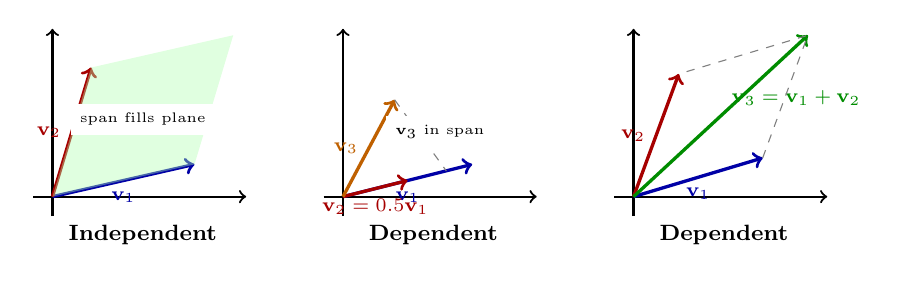
\begin{tikzpicture}[scale=0.82,every node/.style={font=\scriptsize}]
  % independent
  \begin{scope}
    \draw[->,thick] (-0.3,0)--(3.0,0); \draw[->,thick] (0,-0.3)--(0,2.6);
    \draw[->,very thick,blue!65!black] (0,0)--(2.2,0.5) node[midway,below] {$\mathbf{v}_1$};
    \draw[->,very thick,red!65!black] (0,0)--(0.6,2.0) node[midway,left] {$\mathbf{v}_2$};
    \fill[green!30,opacity=0.4] (0,0)--(2.2,0.5)--(2.8,2.5)--(0.6,2.0)--cycle;
    \node[font=\tiny,fill=white] at (1.4,1.2) {span fills plane};
    \node[font=\footnotesize\bfseries] at (1.4,-0.6) {Independent};
  \end{scope}
  % dependent
  \begin{scope}[xshift=4.5cm]
    \draw[->,thick] (-0.3,0)--(3.0,0); \draw[->,thick] (0,-0.3)--(0,2.6);
    \draw[->,very thick,blue!65!black] (0,0)--(2.0,0.5) node[midway,below] {$\mathbf{v}_1$};
    \draw[->,very thick,red!65!black] (0,0)--(1.0,0.25) node[midway,below] {$\mathbf{v}_2=0.5\mathbf{v}_1$};
    \draw[->,very thick,orange!75!black] (0,0)--(0.8,1.5) node[midway,left] {$\mathbf{v}_3$};
    \draw[dashed,gray] (0.8,1.5)--(1.6,0.4);
    \node[font=\tiny,fill=white] at (1.5,1.0) {$\mathbf{v}_3$ in span};
    \node[font=\footnotesize\bfseries] at (1.4,-0.6) {Dependent};
  \end{scope}
  \begin{scope}[xshift=9.0cm]
    \draw[->,thick] (-0.3,0)--(3.0,0); \draw[->,thick] (0,-0.3)--(0,2.6);
    \draw[->,very thick,blue!65!black] (0,0)--(2.0,0.6) node[midway,below] {$\mathbf{v}_1$};
    \draw[->,very thick,red!65!black] (0,0)--(0.7,1.9) node[midway,left] {$\mathbf{v}_2$};
    \draw[->,very thick,green!55!black] (0,0)--(2.7,2.5) node[midway,above right] {$\mathbf{v}_3=\mathbf{v}_1+\mathbf{v}_2$};
    \draw[dashed,gray] (2.0,0.6)--(2.7,2.5)--(0.7,1.9);
    \node[font=\footnotesize\bfseries] at (1.4,-0.6) {Dependent};
  \end{scope}
\end{tikzpicture}
\caption{Left: independent --- new direction each time. Middle/Right: dependent --- one vector lies in the span of the others.}
\label{fig:independence}
\end{figure}

\begin{example}[Polynomials]
In $\mathcal{P}_2$, $\{1,\;x,\;x^2\}$ is independent; $\{1,\;x,\;1+x\}$ is dependent since $(1+x)-1-x=0$. The test is the same: nontrivial coefficients making the zero polynomial.
\end{example}

\section{Span, Basis, Dimension}
\label{sec:basis}
\begin{definition}[Span and basis]
$\operatorname{span}\{\mathbf{v}_1,\dots,\mathbf{v}_k\}$ is the set of all combinations $\sum c_i\mathbf{v}_i$. A \emph{basis} of $V$ is a set that (i) is independent and (ii) spans $V$. The \emph{dimension} $\dim V$ is the number of vectors in any basis (proved well-defined below).
\end{definition}

Bases are not unique, but size is. Coordinates are unique once a basis is fixed.

\begin{theorem}[Dimension well-defined]
Any two bases of a finite-dimensional $V$ have the same cardinality. Any independent set can be extended to a basis; any spanning set contains a basis.
\end{theorem}
\begin{proof}[Sketch]
If $B$ is a basis ($n$ vectors) and $S$ is independent ($k$ vectors), each $\mathbf{s}\in S$ is a unique combination of $B$ --- the coordinate matrix is $n\times k$ with independent columns, so $k\le n$. Symmetrically $n\le k$ when both are bases.
\end{proof}

\begin{figure}[h]
\centering
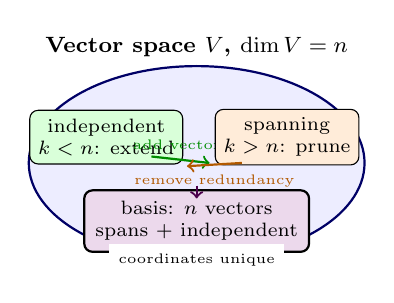
\begin{tikzpicture}[scale=0.82,every node/.style={font=\scriptsize}]
  \draw[rounded corners=4pt,fill=blue!7,draw=blue!40!black,thick] (0,0) ellipse (2.6 and 1.5);
  \node[font=\footnotesize\bfseries] at (0,1.8) {Vector space $V$, $\dim V=n$};
  % independent set
  \node[draw,fill=green!15,rounded corners=3pt,inner sep=3pt,align=center] at (-1.4,0.4) {independent\\$k<n$: extend};
  \draw[->,thick,green!55!black] (-0.7,0.1)--(0.2,0.0) node[midway,above,font=\tiny] {add vectors};
  % spanning set
  \node[draw,fill=orange!15,rounded corners=3pt,inner sep=3pt,align=center] at (1.4,0.4) {spanning\\$k>n$: prune};
  \draw[->,thick,orange!70!black] (0.7,0.0)--(-0.15,-0.05) node[midway,below,font=\tiny] {remove redundancy};
  % basis in middle
  \node[draw,fill=violet!15,rounded corners=3pt,thick,inner sep=4pt,align=center] at (0,-0.9) {basis: $n$ vectors\\spans + independent};
  \draw[->,thick,violet!60!black] (0,-0.35)--(0,-0.55);
  \node[font=\tiny,fill=white] at (0,-1.5) {coordinates unique};
\end{tikzpicture}
\caption{A basis is a minimal spanning set and a maximal independent set; its size is the dimension.}
\label{fig:basis-dimension}
\end{figure}

\section{Bases for the Four Subspaces; Rank--Nullity}
\label{sec:rank-nullity}
For $A\in\mathbb{R}^{m\times n}$ with REF $R$:
\begin{itemize}
    \item $\mathcal{C}(A)$: basis = columns of $A$ at pivot positions of $R$ (not columns of $R$).
    \item $\mathcal{N}(A)$: free variables give one basis vector each (set one free $=1$, rest $0$, solve for pivots).
    \item Row space: nonzero rows of $R$ (or $R^T$ columns).
\end{itemize}
Let $r=\operatorname{rank}(A)=$ number of pivots $=\dim\mathcal{C}(A)=\dim\text{row space}$.

\begin{theorem}[Rank--nullity]
For $A\in\mathbb{R}^{m\times n}$,
\[
  \operatorname{rank}(A)+\operatorname{nullity}(A)=n,\qquad \operatorname{nullity}(A)=\dim\mathcal{N}(A).
\]
Also $\dim\mathcal{N}(A^T)=m-r$. So $r\le\min(m,n)$.
\end{theorem}

\begin{figure}[h]
\centering
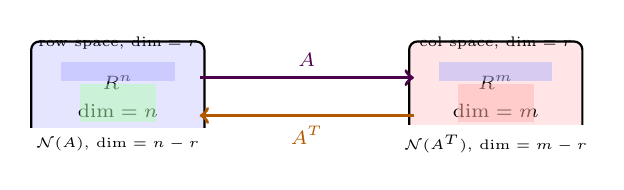
\begin{tikzpicture}[scale=0.80,every node/.style={font=\scriptsize}]
  \node[draw,thick,fill=blue!10,minimum width=2.2cm,minimum height=1.4cm,rounded corners=3pt,align=center] (Rn) at (0,0) {$\mathbb{R}^n$\\[2pt] $\dim=n$};
  \node[draw,thick,fill=red!10,minimum width=2.2cm,minimum height=1.4cm,rounded corners=3pt,align=center] (Rm) at (6.0,0) {$\mathbb{R}^m$\\[2pt] $\dim=m$};
  \draw[->,very thick,violet!60!black] (1.3,0.3)--(4.7,0.3) node[midway,above] {$A$};
  \draw[->,very thick,orange!70!black] (4.7,-0.3)--(1.3,-0.3) node[midway,below] {$A^T$};
  \fill[green!30,opacity=0.5] (-0.6,-0.4) rectangle (0.6,0.2) node[midway,font=\tiny] {};
  \node[font=\tiny,fill=white] at (0,-0.75) {$\mathcal{N}(A)$, $\dim=n-r$};
  \fill[blue!30,opacity=0.5] (-0.9,0.25) rectangle (0.9,0.55);
  \node[font=\tiny] at (0,0.85) {row space, $\dim=r$};
  \fill[blue!30,opacity=0.5] (5.1,0.25) rectangle (6.9,0.55);
  \node[font=\tiny] at (6.0,0.85) {col space, $\dim=r$};
  \fill[red!30,opacity=0.5] (5.4,-0.4) rectangle (6.6,0.2);
  \node[font=\tiny,fill=white] at (6.0,-0.75) {$\mathcal{N}(A^T)$, $\dim=m-r$};
\end{tikzpicture}
\caption{The four subspaces and their dimensions. The row and column spaces both have dimension $r=\operatorname{rank}(A)$.}
\label{fig:four-dims}
\end{figure}

\begin{example}[Rank--nullity in action]
$A=\begin{bmatrix}1&2&1&0\\2&4&3&1\\1&2&2&1\end{bmatrix}\xrightarrow{\text{REF}}
\begin{bmatrix}1&2&1&0\\0&0&1&1\\0&0&0&0\end{bmatrix}$. Pivots in cols $1,3$ so $r=2$, nullity $=4-2=2$. $\mathcal{C}(A)$ basis: cols $1,3$ of $A$; $\mathcal{N}(A)$ basis: from $x_2,x_4$ free.
\end{example}

\begin{example}[Coordinates and change of basis]
Fix basis $B=\{\mathbf{b}_1,\mathbf{b}_2\}$. Then $[\mathbf{v}]_B$ solves $[\mathbf{b}_1\ \mathbf{b}_2][\mathbf{v}]_B=\mathbf{v}$. If $C$ is another basis, $[\mathbf{v}]_C=P_{C\gets B}[\mathbf{v}]_B$ where $P$ has columns $[\mathbf{b}_j]_C$.
\begin{lstlisting}[language=Python]
import numpy as np
B = np.array([[1.,1.],[0.,1.]]).T  # columns are b1,b2 -- careful with layout
# Actually B_cols = [[1,0],[1,1]] as columns
B_cols = np.array([[1.,1.],[0.,1.]])  # col j = B_cols[:,j]
v = np.array([3.,2.])
coords = np.linalg.solve(B_cols, v)
print(coords)  # [1., 2.] meaning v = 1*b1 + 2*b2
print(B_cols @ coords)  # [3., 2.] check
\end{lstlisting}
\end{example}

% ============================================================

% --- Additional depth: Exchange lemma, dimension theorem, and matrix rank ---
\section{Exchange and Dimension Uniqueness}
\label{sec:exchange}
\begin{lemma}[Steinitz exchange]
If $\{\mathbf{v}_1,\dots,\mathbf{v}_n\}$ spans $V$ and $\{\mathbf{u}_1,\dots,\mathbf{u}_k\}$ is independent, then $k\le n$ and the span can exchange $k$ of the $\mathbf{v}_i$ for the $\mathbf{u}_j$ and still span.
\end{lemma}
Corollary: all bases have the same size; any independent set extends to a basis (keep adding vectors outside the current span until spanning); any spanning set prunes to a basis (drop dependent vectors one by one). This justifies calling $\dim V$ well-defined.

\begin{example}[Extending in $\mathcal{P}_2$]
$\{\mathbf{v}_1=1+x\}$ independent in $\mathcal{P}_2$ ($\dim3$) extends to a basis, e.g.\ $\{1+x,\;x,\;x^2\}$ or $\{1+x,\;1-x,\;x^2\}$. Infinitely many bases; dimension is the invariant.
\end{example}

\section{Matrix Rank = Row Rank = Column Rank}
\label{sec:rank-equal}
A nontrivial theorem: $\dim\mathcal{C}(A)=\dim\mathcal{C}(A^T)$ --- column rank equals row rank, both $=r$. So REF pivot count is intrinsic, not an artefact. Proof sketch: show $\mathcal{N}(A)$ is orthogonal complement of row space (Ch.~6); then rank--nullity gives equality.

\section{Change of Basis and Similarity Preview}
\label{sec:change-basis-detail}
If $B$ and $C$ are bases, $P_{C\gets B}$ (columns $[\mathbf{b}_j]_C$) converts $[\mathbf{v}]_B$ to $[\mathbf{v}]_C$. For a linear operator $T:V\to V$, its matrices satisfy $[T]_C=P[T]_BP^{-1}$ --- similarity. Determinant, trace, eigenvalues are similarity invariants (Ch.~7--8). This is why diagonalization $A=PDP^{-1}$ is a change to the eigenbasis where $T$ acts diagonally.


\section{Chapter Notes}
Grassmann (1844) first framed dimension this way. Rank--nullity is the ``conservation of dimensions'' for $A:\mathbb{R}^n\to\mathbb{R}^m$. Computing rank via SVD (Ch.~6/8 notes) is numerically stable; REF rank is exact-arithmetic.

% ============================================================
\section{Exercises}
\label{sec:ch05-exercises}
\begin{enumerate}[label=E5.\arabic*, leftmargin=*, itemsep=0.8em]
\item \textbf{Test.} Are $\mathbf{v}_1=[1,0,1]^T$, $\mathbf{v}_2=[0,1,1]^T$, $\mathbf{v}_3=[1,1,2]^T$ independent? If dependent, write one as a combination of the others.
\item \textbf{Bases from REF.} For $A=\begin{bmatrix}1&2&0&1\\0&0&1&2\\1&2&1&3\end{bmatrix}$, find bases for $\mathcal{C}(A)$, $\mathcal{N}(A)$, and row space. Verify rank$+$nullity$=n$ and $r\le\min(m,n)$.
\item \textbf{Coordinates.} Let $B=\{[1,1]^T,[1,-1]^T\}$ be a basis of $\mathbb{R}^2$. Find $[\mathbf{v}]_B$ for $\mathbf{v}=[3,1]^T$. If $C$ is the standard basis, write $P_{C\gets B}$ and $P_{B\gets C}$.
\item \textbf{Dimension bound.} Prove any $k>n$ vectors in $\mathbb{R}^n$ are dependent. Deduce $\dim\mathbb{R}^n=n$ via the standard basis.
\item \textbf{Coding.} Write \texttt{col\_basis(A)} returning indices of pivot columns (tolerance $10^{-10}$) and a basis for $\mathcal{N}(A)$ via SVD or REF. Compare with \texttt{scipy.linalg.null\_space} on random $5\times7$ matrices.
\end{enumerate}
% End of Chapter 5
